\documentclass[11pt]{article}

\usepackage{listings}
\usepackage{graphicx}
\usepackage{titling}
\usepackage{fullpage}
\newcommand{\subtitle}[1]{%
  \posttitle{%
    \par\end{center}
    \begin{center}\large#1\end{center}
    \vskip0.5em}%
}

%%\renewcommand{\topfraction}{0.9}    % max fraction of floats at top
%%\renewcommand{\bottomfraction}{0.8}

\begin{document}

\title{Deeva}
\subtitle{Planing Report}
\author{Kritaphat Sonsri-in, Xueqi Chen, Hector Dearman, \\Alina Draganescu, Felix De Souza}

\maketitle

\section{The Task}
Our group was assigned to a project to build a simple but powerful Java debugger to help teach first year computing students Java.

Our supervisor Dr.~Tristan Allwood proposed this project for two main reasons.
Firstly although he would like to avoid teaching Java in a way that made students dependent on a `magic' IDE like Eclipse this becomes difficult without a good external debugger like GDB is for C\footnote{The various external Java debuggers like JDB all have serious bugs and/or usability problems.}.
Secondly many students initially don't have a clear mental picture of what the computer is doing\footnote{Roughly half are programing in an imperative language for the first time.} so it would be good for students to be able to graphically inspect the stack and heap of a running Java program in a similar way to how they are being taught to visualize the stack and heap in lectures.

To fix these problems he envisioned a Java debugger that was: started from the command line (to avoid IDE magic), intuitive enough to used by people who had not previously used a debugger (but powerful enough to be useful) and which could visually display the state of the stack and the heap to help further the development of a mental model of Java.

%%After we discussed with , who proposed this project, we understood that the problem while teaching Java to first year students is that students tend to get really dependant on IDE like Eclipse with functionalities like auto-fill etc. Tristan has tried alternatives like using JDB however it sometimes gets out of sync and breaks. This is why he wants a simpler version of IDE that is more light-weight.

\section{How we prepared the Plan}

For this project we have three problems which we don't normally have in university project: we're not sure what we're building, we want to make sure we deliver the software on time but don't know how long it will take and
we want to make sure the software we write is correct and useful but have no easy way to define `correct' or `useful' in this domain.

Happily Agile programing was designed to solve these problems xxx

\subsection{Requirement Analysis}
As stated in the article \textit{Requirements analysis}\footnote{\tt{http://en.wikipedia.org/wiki/Requirements\_analysis}}, requirements analysis conceptually includes three types of activities: requirements gathering, analyzing requirements, and recording requirements.
Following this approch, we had an internal meeting, firstly, to identify stakeholders which involve first year students; Tristan, our project owner; lab helpers; and CSG, who will deploy our project to lab machines. Then, we discussed and shared common understanding of the project. We initialised a list of requirements by researching on debuggers to see the already-exist features. Subsequently, we made an appointment with Tristan to discuss our approach on the project. Regarding the meeting with Tristan, we agreed on our requirements, and Tristan prioritised the features of the debugger. Then we came up with a release plan. In addition, we also considered use cases by using first year tutorials and lab exercised as a refference. After the requirement gathering step, we had a second meeting with Tristan to make a clear final decision concerning core requirements and feature priorities. And, we used contract-style requirement list\footnote{\tt{http://en.wikipedia.org/wiki/Requirements\_analysis\#Contract-style\_requirement\_lists}} to provide a contract between us.
Any change made in the plan and requirements were recorded and updated using Google Drive. Major changes were made after the first meeting with Tristan; only slight change was made after the second meeting.
All requirements and changes are displayed in the project plan.

\subsection{First Group Meeting}
After our first meeting with Tristan, we had our first formal group meeting with the information Tristan had provided us. We decided to use Agile Programming as we go along. During the meeting, we came up with some research topics that were neccessary for the project such as: tools/frameworks, different java debugger comparison, getting first year java projects and etc. Everyone picked one story base on their preference with a set deadline. For example, Krit and Kira were working on the comparison of different debuggers, we used google docs for editing and gathering information that we had found. Hector and Felix were working on researching on frameworks. Alina was assigned with making estimation pokers and getting the first year java projects. 
\begin{figure}[h!]
\centering
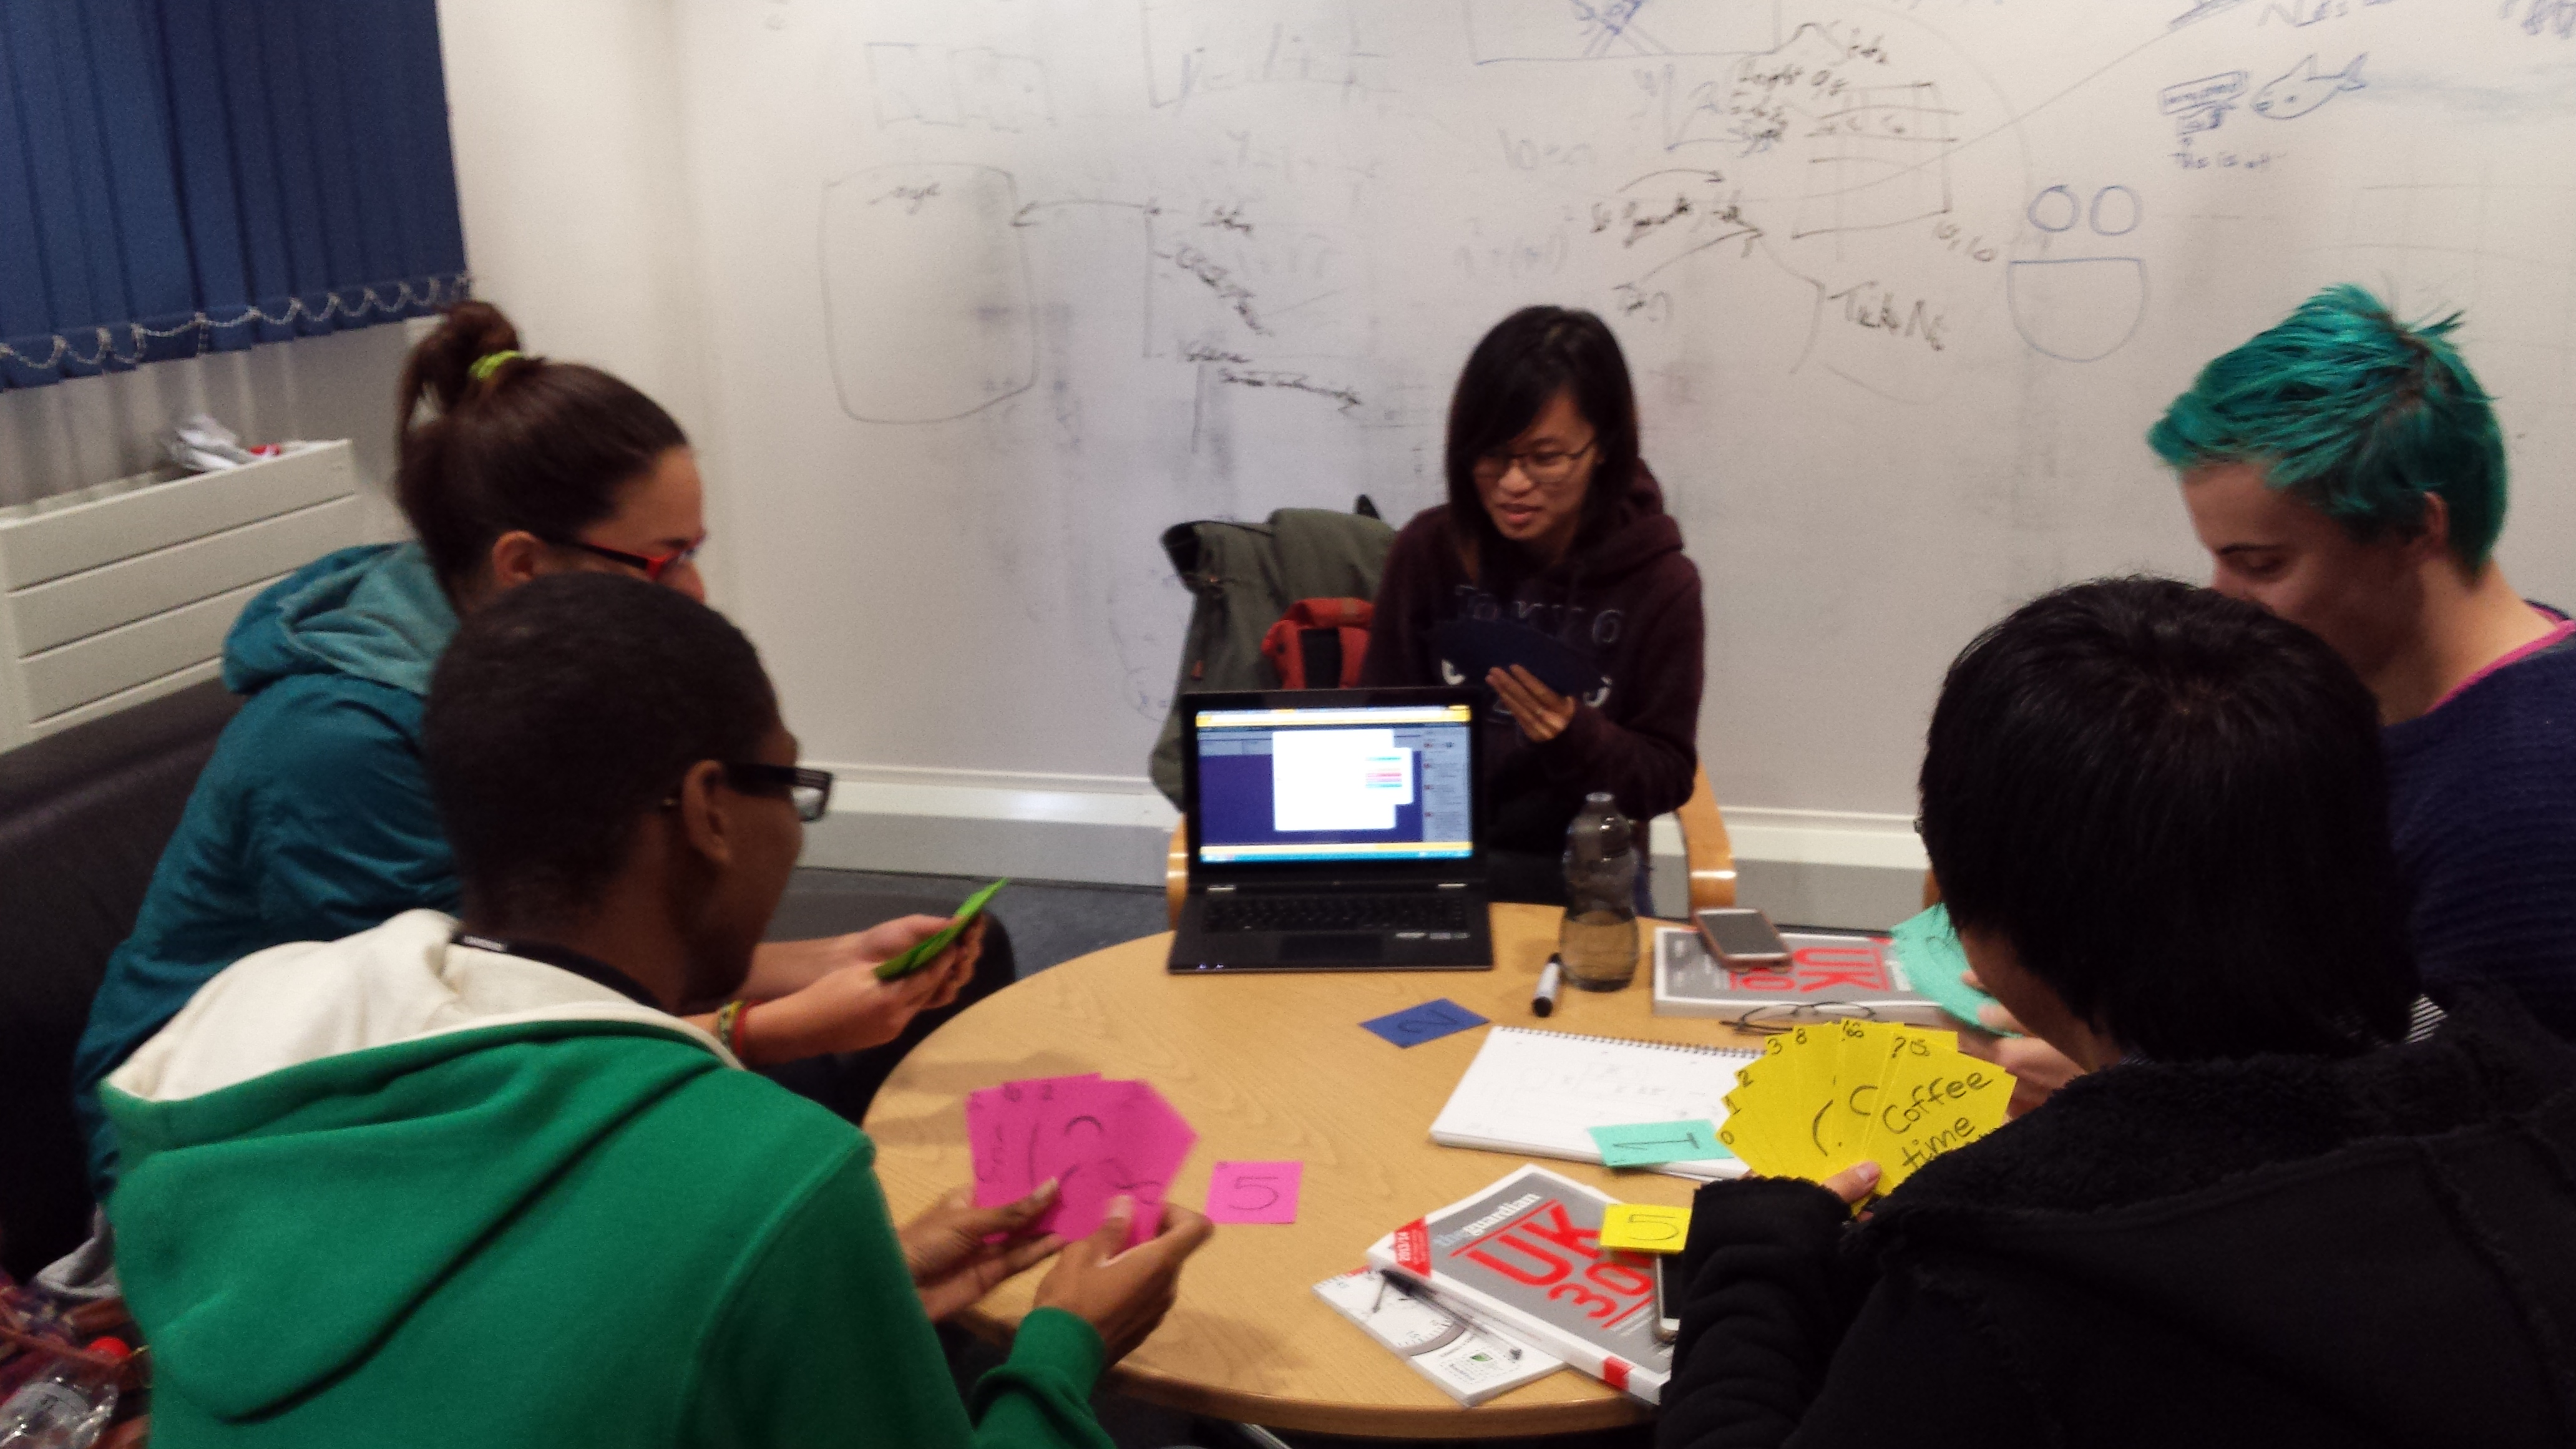
\includegraphics[width=110mm]{estimation.jpg}
\end{figure}  

\subsection{Second Group Meeting}
In our second group meeting we discussed the research results from the previous iteration. We decided which tools would best fit our requirements and would be easy to integrate between each other. Afterwards, we created a formal plan that covers: iteration-by-iteration, all the milestones needed to deliver the product in time. For example, by week 5 we plan to have a minimal-feature demo to show Tristan and by week 7 we plan to have a basic-feature debugger that can get tested by first year students starting the `Intro to Java' course. Finally, we created new stories for each stub part of our minimal implementation. Again, we used Planning Poker to estimate the stories and then allocate them to a memeber of the team. For example, the card 'Front end' got a score of 3 and got allocated to Krit. 

\section{Our Plan}

We elected to write a very simple plan to avoid wasting a lot of time on something that ``wouldn't survive contact with the enemy" and give us more time to iterate. 
Of course if our plan was too vague it would be useless so we had to strike a balance.
In the end our plan contained the essentials: a strong statement of the requirements (both minimum and extensions), a week by week work timetable of what we hoped to achieve, an overview of the architecture we are using and a description of the process we are using to build the software.


\section{Tools}

\begin{description}
  \item[Trello] \hfill \\
  As an Information Radiator\footnote{\tt{https://www.atlassian.com/wallboards/information-radiators.jsp}} we decided to use an electronic version, Trello, which allows us to track our progress and average velocity. We decided to use Trello as it fulfills most of the key features required for such a tool: it is easy to use and update, relatively flexible and allows for communications between members without to much interruption\footnote{\tt{https://www.atlassian.com/wallboards/information-radiators.jsp}}. Electronic notice boards are a manageable alternative to physical boards and we found it extremely useful when it came to keeping everyone informed on the general progress and keeping all the information in one compact environment. 
  A Trello board was created for a better project management process. There are several different swimlanes on the board: ``Proposed'', which allows all members to throw in ideas; ``In analysis'', where people talk about their ideas and have a discussion with group members to see if the story is feasible. If it is, the card will be then moved to ``In estimation'' where we gather together to use planning pokers to give a complexity points to the story. Otherwise, the story will be moved to ``Discarded''. The reason why we want to keep track of what we have discarded is that we might have thought we would not have time for it but in reality we did have time at the end, we might want to move it back and reconsider it. After estimation, the card will be assigned to group members with a set due date and be moved into ``In development'' on the Trello board. Once the development is complete, the card should be moved into ``In review''. This is when we need someone to review our code to improve our styling and pattern-usage.  
\begin{figure}[h!]
\centering
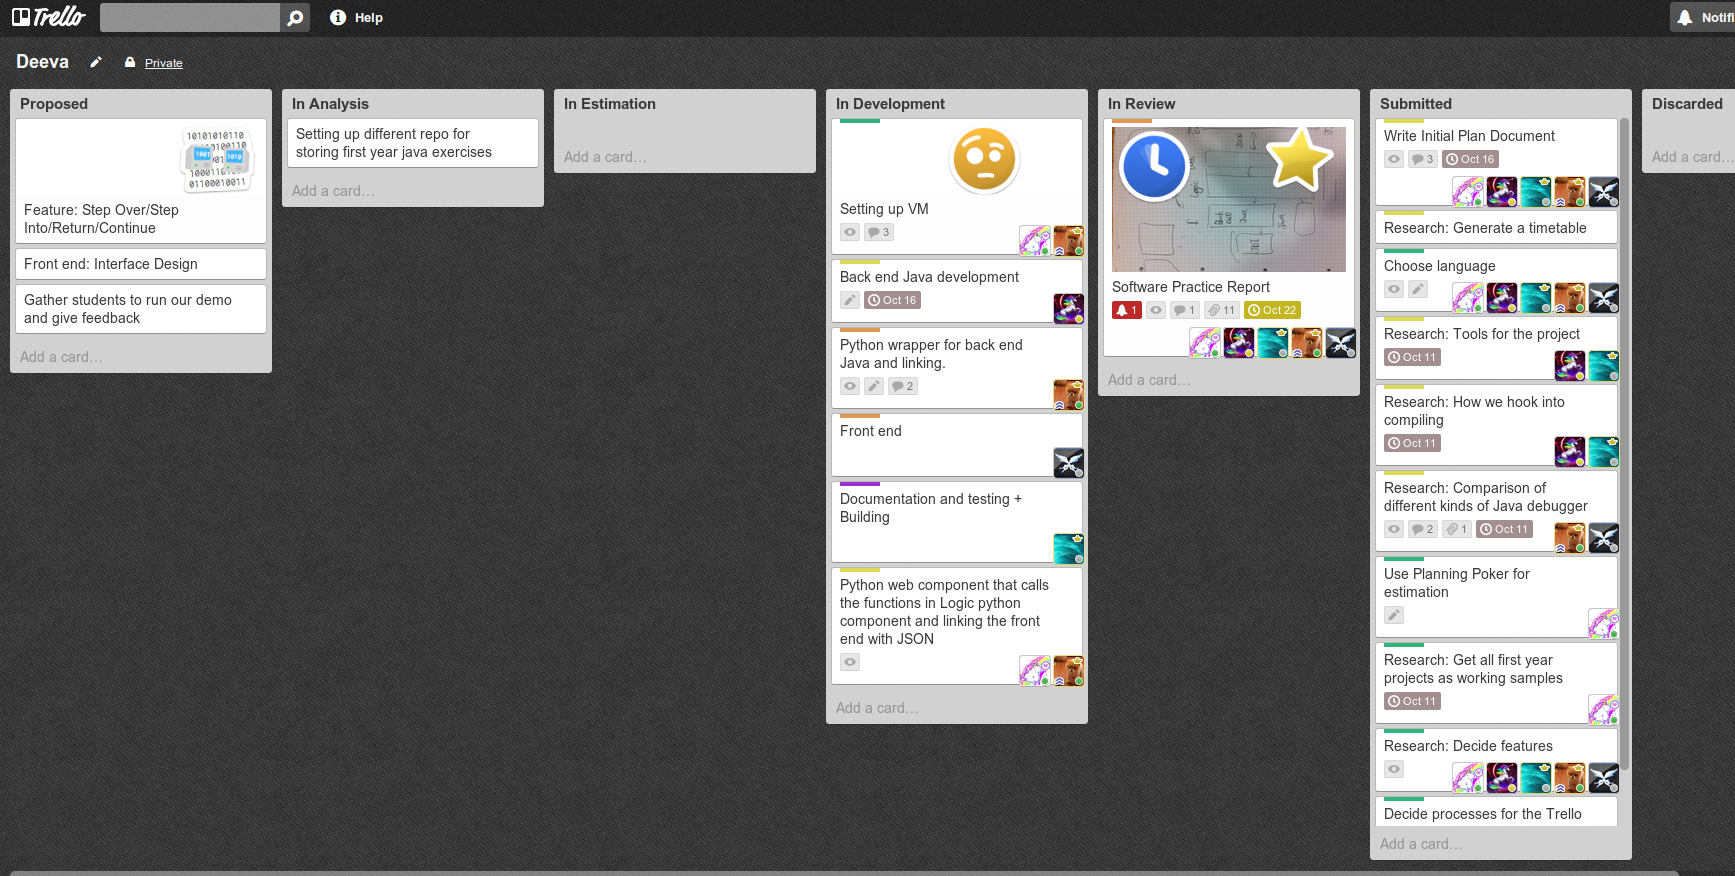
\includegraphics[width=\textwidth]{Trello.png}
\end{figure}
  \item[Planing Poker] \hfill \\
We are using Planning Poker in order to estimate stories in each cycle of development. This method is known to avoid anchoring and will produce more accurate, less optimistic story point estimations\footnote{\tt{http://en.wikipedia.org/wiki/Planning\_poker\#Planning\_poker\_benefits}}. This technique takes some time to get used to because initially the story point bared little meaning to us. As the tasks got more concrete and we got used to compare stories against numbers in the fibonacci sequence the poker game proved to be a very efficient method. 
For example, it helped determine when people aren't really talking about the same scope for a certain task. Frequently we have a task like ``Set up the back end." and one person gives a task a 2 while another gives it an 8. The first person thinks the task title means ``Write some stubs so the middleware can integrate." while the second thinks it means ``Implement the backend up to the minimal specification.". So using planing poker has already helped us make sure we're all on the same page. One of our group members had hand-made a set of pokers just for estimation. It contains Fibonacci number 0 - 13 and ``infinity'' if we think it's impossible to do as well as ``coffee time'' if we think we need a break. 
\begin{figure}[h!]
\centering
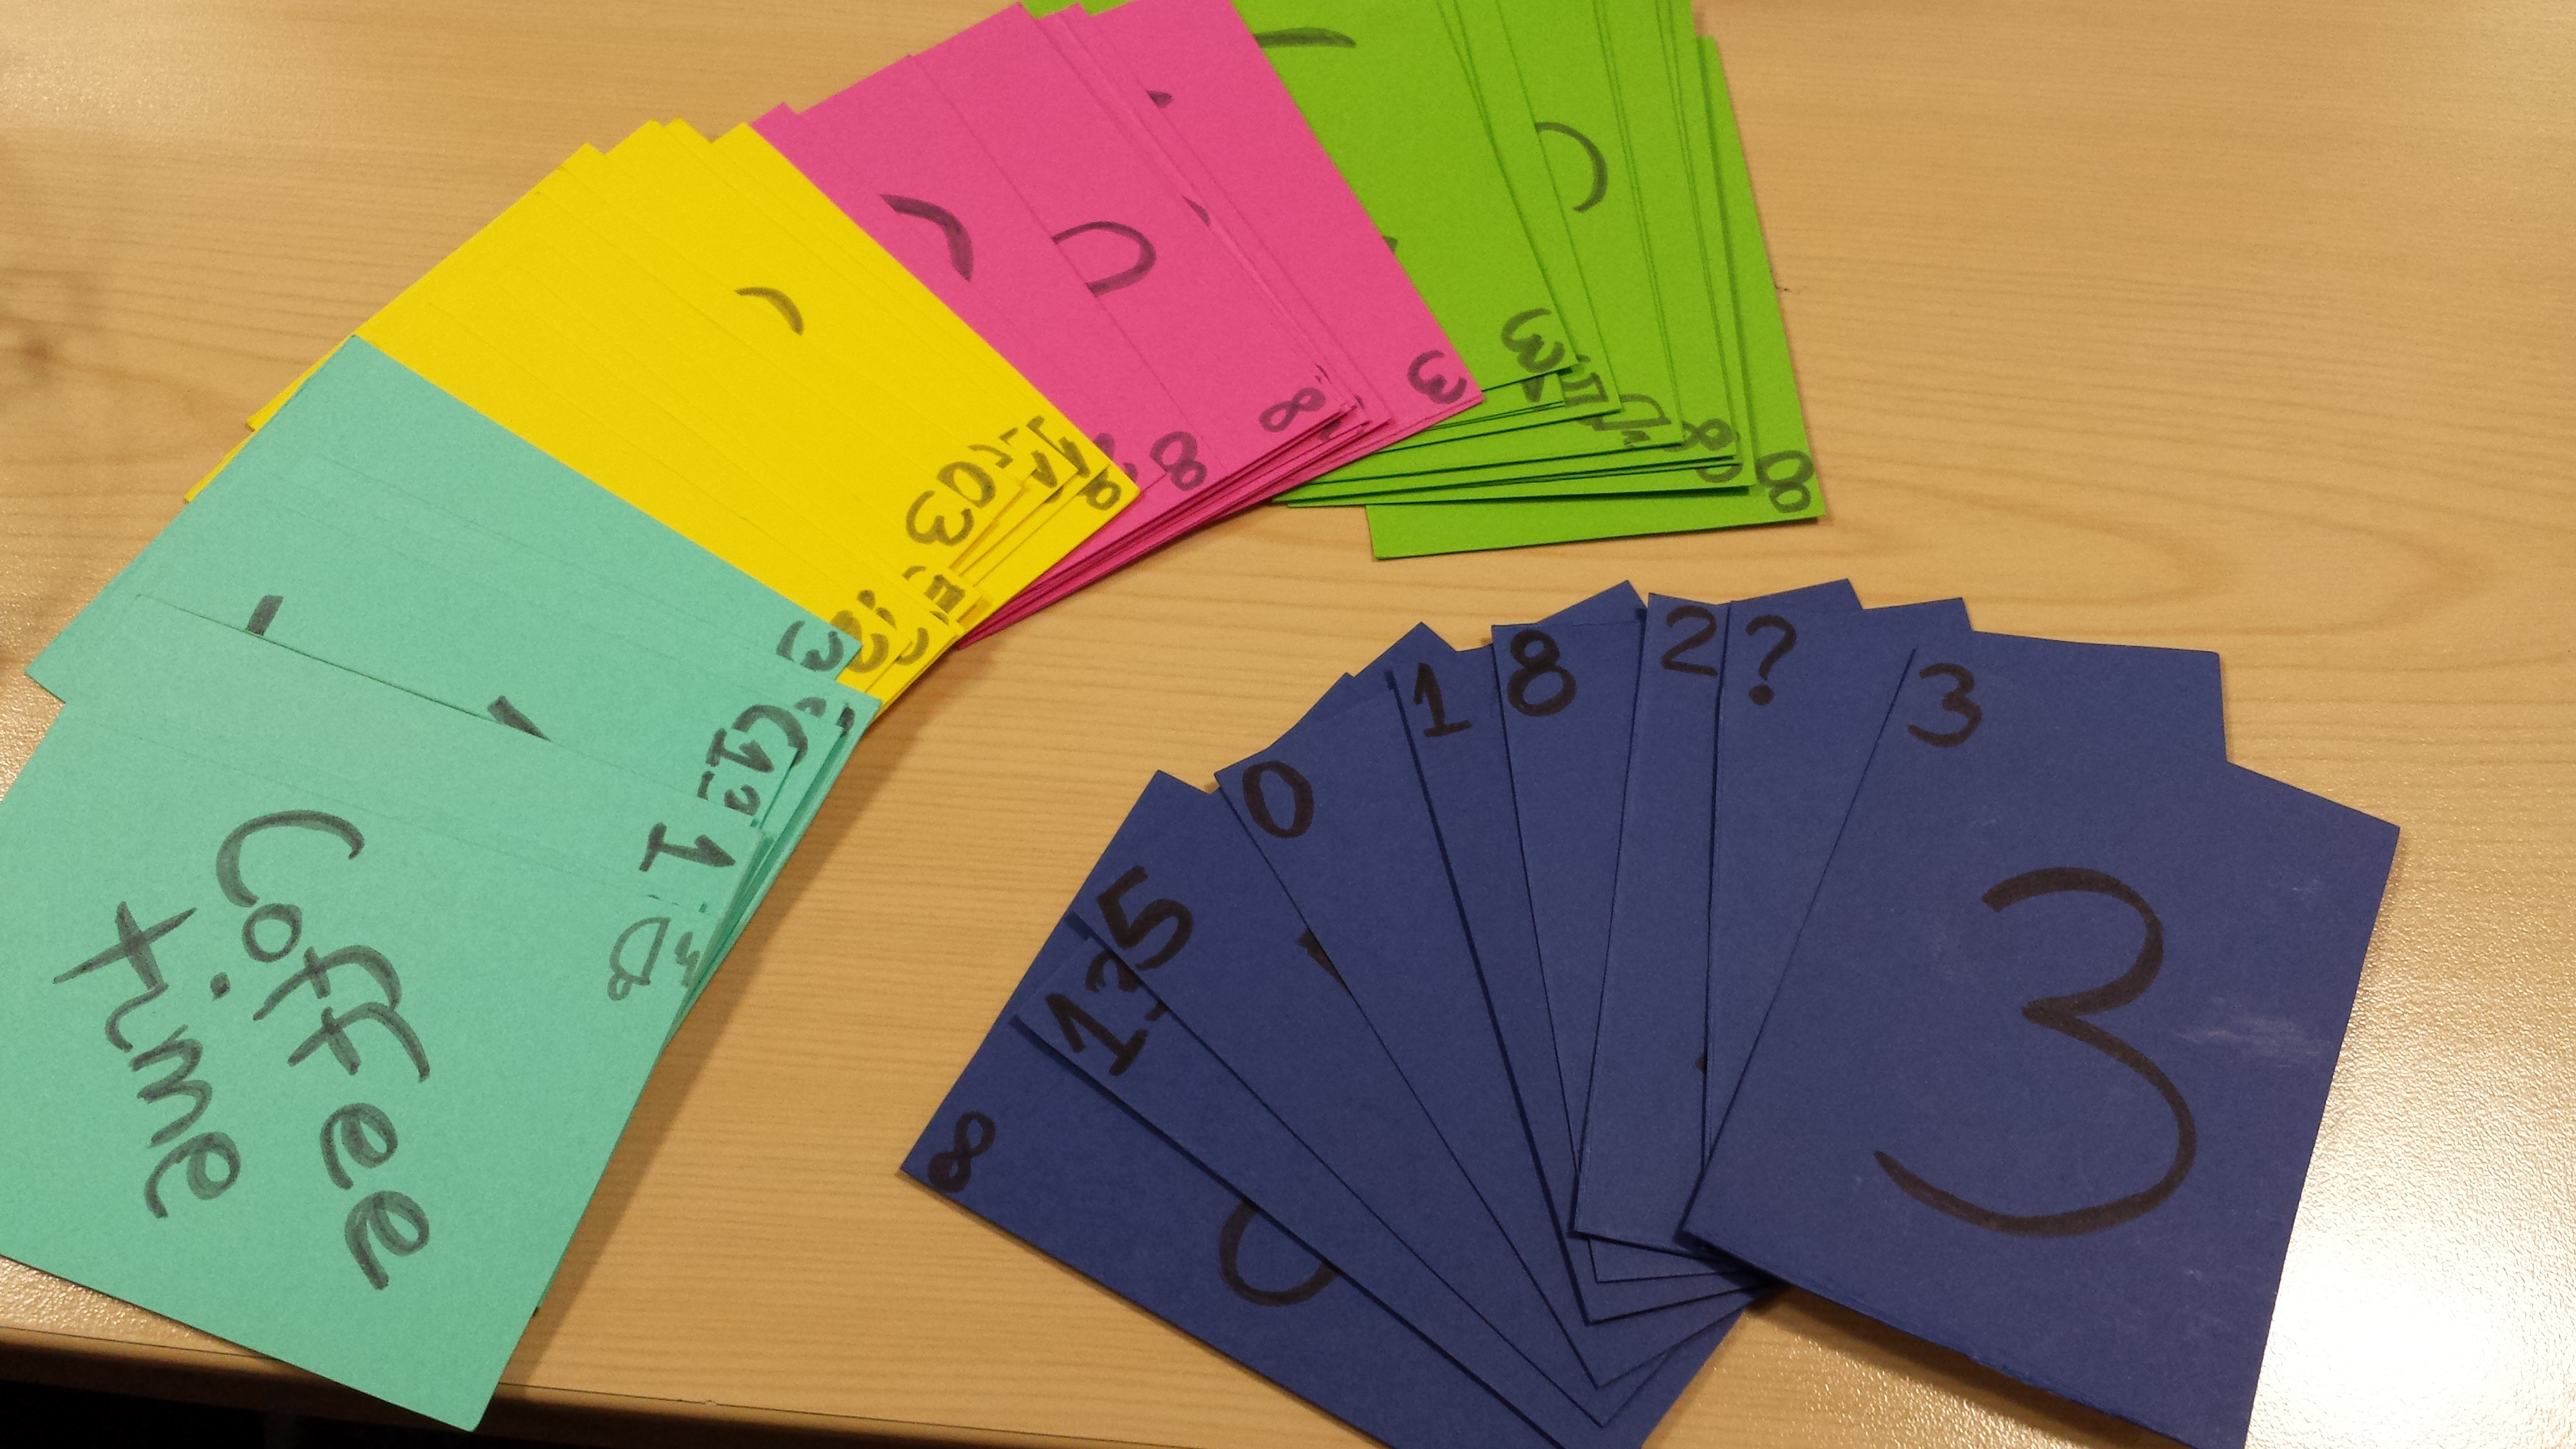
\includegraphics[width=100mm]{planningPokers.jpg}
\end{figure}  
  \item[Facebook Group] \hfill \\
  For questions and comment that are too general or conversational for Trello.
  \item[Google Docs] \hfill \\
  For collaborative editing on reports and plans.
  \item[Github] \hfill \\
  Source control which somebody else manages and is easily accessible from anywhere
  (which also plays nice with tools like Travis).


\end{description}


\end{document}
